% Queue wide assets early so they can appear beside the experimental discussion.
\begin{table}[t]
\caption{MIRA configuration shared across motions.}
\label{tab:config}
\centering\small
\setlength{\tabcolsep}{3.5pt}
\begin{tabular}{ll}
\toprule
Component & Setting \\
\midrule
Physical error input & $64$ components, $7$ groups \\
Energy network & $64\to341\to512\to1$ \\
Activation & MixedELU \\
Linear maps & nonnegative, diagonal-normalized \\
Input normalization & group scale and $\sqrt{d_g}$ scaling \\
Scale statistics & fixed after $10^8$ samples \\
Actor / value network & MLP, hidden widths $1024$, $512$ \\
Actor / value optimizer & SGD, lr $10^{-4}$ \\
Discriminator optimizer & SGD, lr $2.5\times10^{-4}$ \\
PPO settings & $\gamma=0.99$, GAE $0.95$, clip $0.2$ \\
Replay capacity & $2\times10^5$ samples \\
Output-weight regularizer & $0.01$ \\
Gradient penalty & $0$ \\
\bottomrule
\end{tabular}
\end{table}

% Generated by PAPER/tools/build_mira_experiments.py; do not hand-edit.
\begin{table*}[t]
\caption{Tracking errors at the common 2000-update budget. (a) Equal-weight
macro-averages over all six motions; incomplete aggregates remain TODO.
(b) Available MIRA motion results and pending entries. Lower is better.
\textcolor{orange!70!black}{$\dagger$: Random layout deviations, not measured
seed variability; centers retain the measured seed-0 values.}
Climb$^\ddagger$ uses the 2000-update checkpoint, before its extension;
its evaluation terminates early. Errors cover executed timesteps.}
\label{tab:main}
\centering\small
\setlength{\tabcolsep}{8pt}
\textbf{(a) Six-motion macro-average}\\[2pt]
\begin{tabular}{lcccc}\toprule
Metric $\downarrow$ & AMP & DeepMimic & ADD & MIRA \\
\midrule
Root pos. [m] & $0.4704\!\pm\!\textcolor{orange!70!black}{0.0185}^{\dagger}$ & $0.0665\!\pm\!\textcolor{orange!70!black}{0.0029}^{\dagger}$ & $0.0683\!\pm\!\textcolor{orange!70!black}{0.0046}^{\dagger}$ & \tbd \\
Root rot. [rad] & $0.7697\!\pm\!\textcolor{orange!70!black}{0.0337}^{\dagger}$ & $0.1297\!\pm\!\textcolor{orange!70!black}{0.0036}^{\dagger}$ & $0.0640\!\pm\!\textcolor{orange!70!black}{0.0032}^{\dagger}$ & \tbd \\
Body pos. [m] & $0.2090\!\pm\!\textcolor{orange!70!black}{0.0067}^{\dagger}$ & $0.0488\!\pm\!\textcolor{orange!70!black}{0.0034}^{\dagger}$ & $0.0335\!\pm\!\textcolor{orange!70!black}{0.0016}^{\dagger}$ & \tbd \\
Body rot. [rad] & $0.7929\!\pm\!\textcolor{orange!70!black}{0.0430}^{\dagger}$ & $0.1950\!\pm\!\textcolor{orange!70!black}{0.0093}^{\dagger}$ & $0.1254\!\pm\!\textcolor{orange!70!black}{0.0059}^{\dagger}$ & \tbd \\
DoF vel. [rad/s] & $1.4224\!\pm\!\textcolor{orange!70!black}{0.0577}^{\dagger}$ & $0.8684\!\pm\!\textcolor{orange!70!black}{0.0381}^{\dagger}$ & $0.6762\!\pm\!\textcolor{orange!70!black}{0.0314}^{\dagger}$ & \tbd \\
Root vel. [m/s] & $0.4178\!\pm\!\textcolor{orange!70!black}{0.0111}^{\dagger}$ & $0.1712\!\pm\!\textcolor{orange!70!black}{0.0060}^{\dagger}$ & $0.1958\!\pm\!\textcolor{orange!70!black}{0.0078}^{\dagger}$ & \tbd \\
Root ang. vel. [rad/s] & $1.0090\!\pm\!\textcolor{orange!70!black}{0.0472}^{\dagger}$ & $0.4162\!\pm\!\textcolor{orange!70!black}{0.0217}^{\dagger}$ & $0.3822\!\pm\!\textcolor{orange!70!black}{0.0162}^{\dagger}$ & \tbd \\
\bottomrule\end{tabular}
\par\vspace{5pt}
\textbf{(b) MIRA motion coverage}\\[2pt]
\scriptsize
\setlength{\tabcolsep}{3.5pt}
\resizebox{\textwidth}{!}{\begin{tabular}{lccccccc}\toprule
Motion & Root pos. & Root rot. & Body pos. & Body rot. & DoF vel. & Root vel. & Root ang. vel. \\
\midrule
Roll & \tbd & \tbd & \tbd & \tbd & \tbd & \tbd & \tbd \\
Climb$^\ddagger$ & $0.1607\!\pm\!\textcolor{orange!70!black}{0.0012}^{\dagger}$ & $0.0712\!\pm\!\textcolor{orange!70!black}{0.00002}^{\dagger}$ & $0.0412\!\pm\!\textcolor{orange!70!black}{0.0018}^{\dagger}$ & $0.1615\!\pm\!\textcolor{orange!70!black}{0.0065}^{\dagger}$ & $0.8521\!\pm\!\textcolor{orange!70!black}{0.0413}^{\dagger}$ & $0.3132\!\pm\!\textcolor{orange!70!black}{0.0155}^{\dagger}$ & $0.4652\!\pm\!\textcolor{orange!70!black}{0.0251}^{\dagger}$ \\
Backflip & $0.0544\!\pm\!\textcolor{orange!70!black}{0.0033}^{\dagger}$ & $0.0303\!\pm\!\textcolor{orange!70!black}{0.0026}^{\dagger}$ & $0.0373\!\pm\!\textcolor{orange!70!black}{0.0023}^{\dagger}$ & $0.1701\!\pm\!\textcolor{orange!70!black}{0.0073}^{\dagger}$ & $0.9793\!\pm\!\textcolor{orange!70!black}{0.0425}^{\dagger}$ & $0.2760\!\pm\!\textcolor{orange!70!black}{0.0133}^{\dagger}$ & $0.2316\!\pm\!\textcolor{orange!70!black}{0.0098}^{\dagger}$ \\
Crawl & $0.0074\!\pm\!\textcolor{orange!70!black}{0.0006}^{\dagger}$ & $0.0075\!\pm\!\textcolor{orange!70!black}{0.0004}^{\dagger}$ & $0.0065\!\pm\!\textcolor{orange!70!black}{0.0002}^{\dagger}$ & $0.0356\!\pm\!\textcolor{orange!70!black}{0.0013}^{\dagger}$ & $0.1735\!\pm\!\textcolor{orange!70!black}{0.0080}^{\dagger}$ & $0.0267\!\pm\!\textcolor{orange!70!black}{0.0009}^{\dagger}$ & $0.0672\!\pm\!\textcolor{orange!70!black}{0.0041}^{\dagger}$ \\
Get-Up & \tbd & \tbd & \tbd & \tbd & \tbd & \tbd & \tbd \\
Spin Kick & \tbd & \tbd & \tbd & \tbd & \tbd & \tbd & \tbd \\
\bottomrule\end{tabular}}
\end{table*}


\begin{figure*}[!t]
\centering
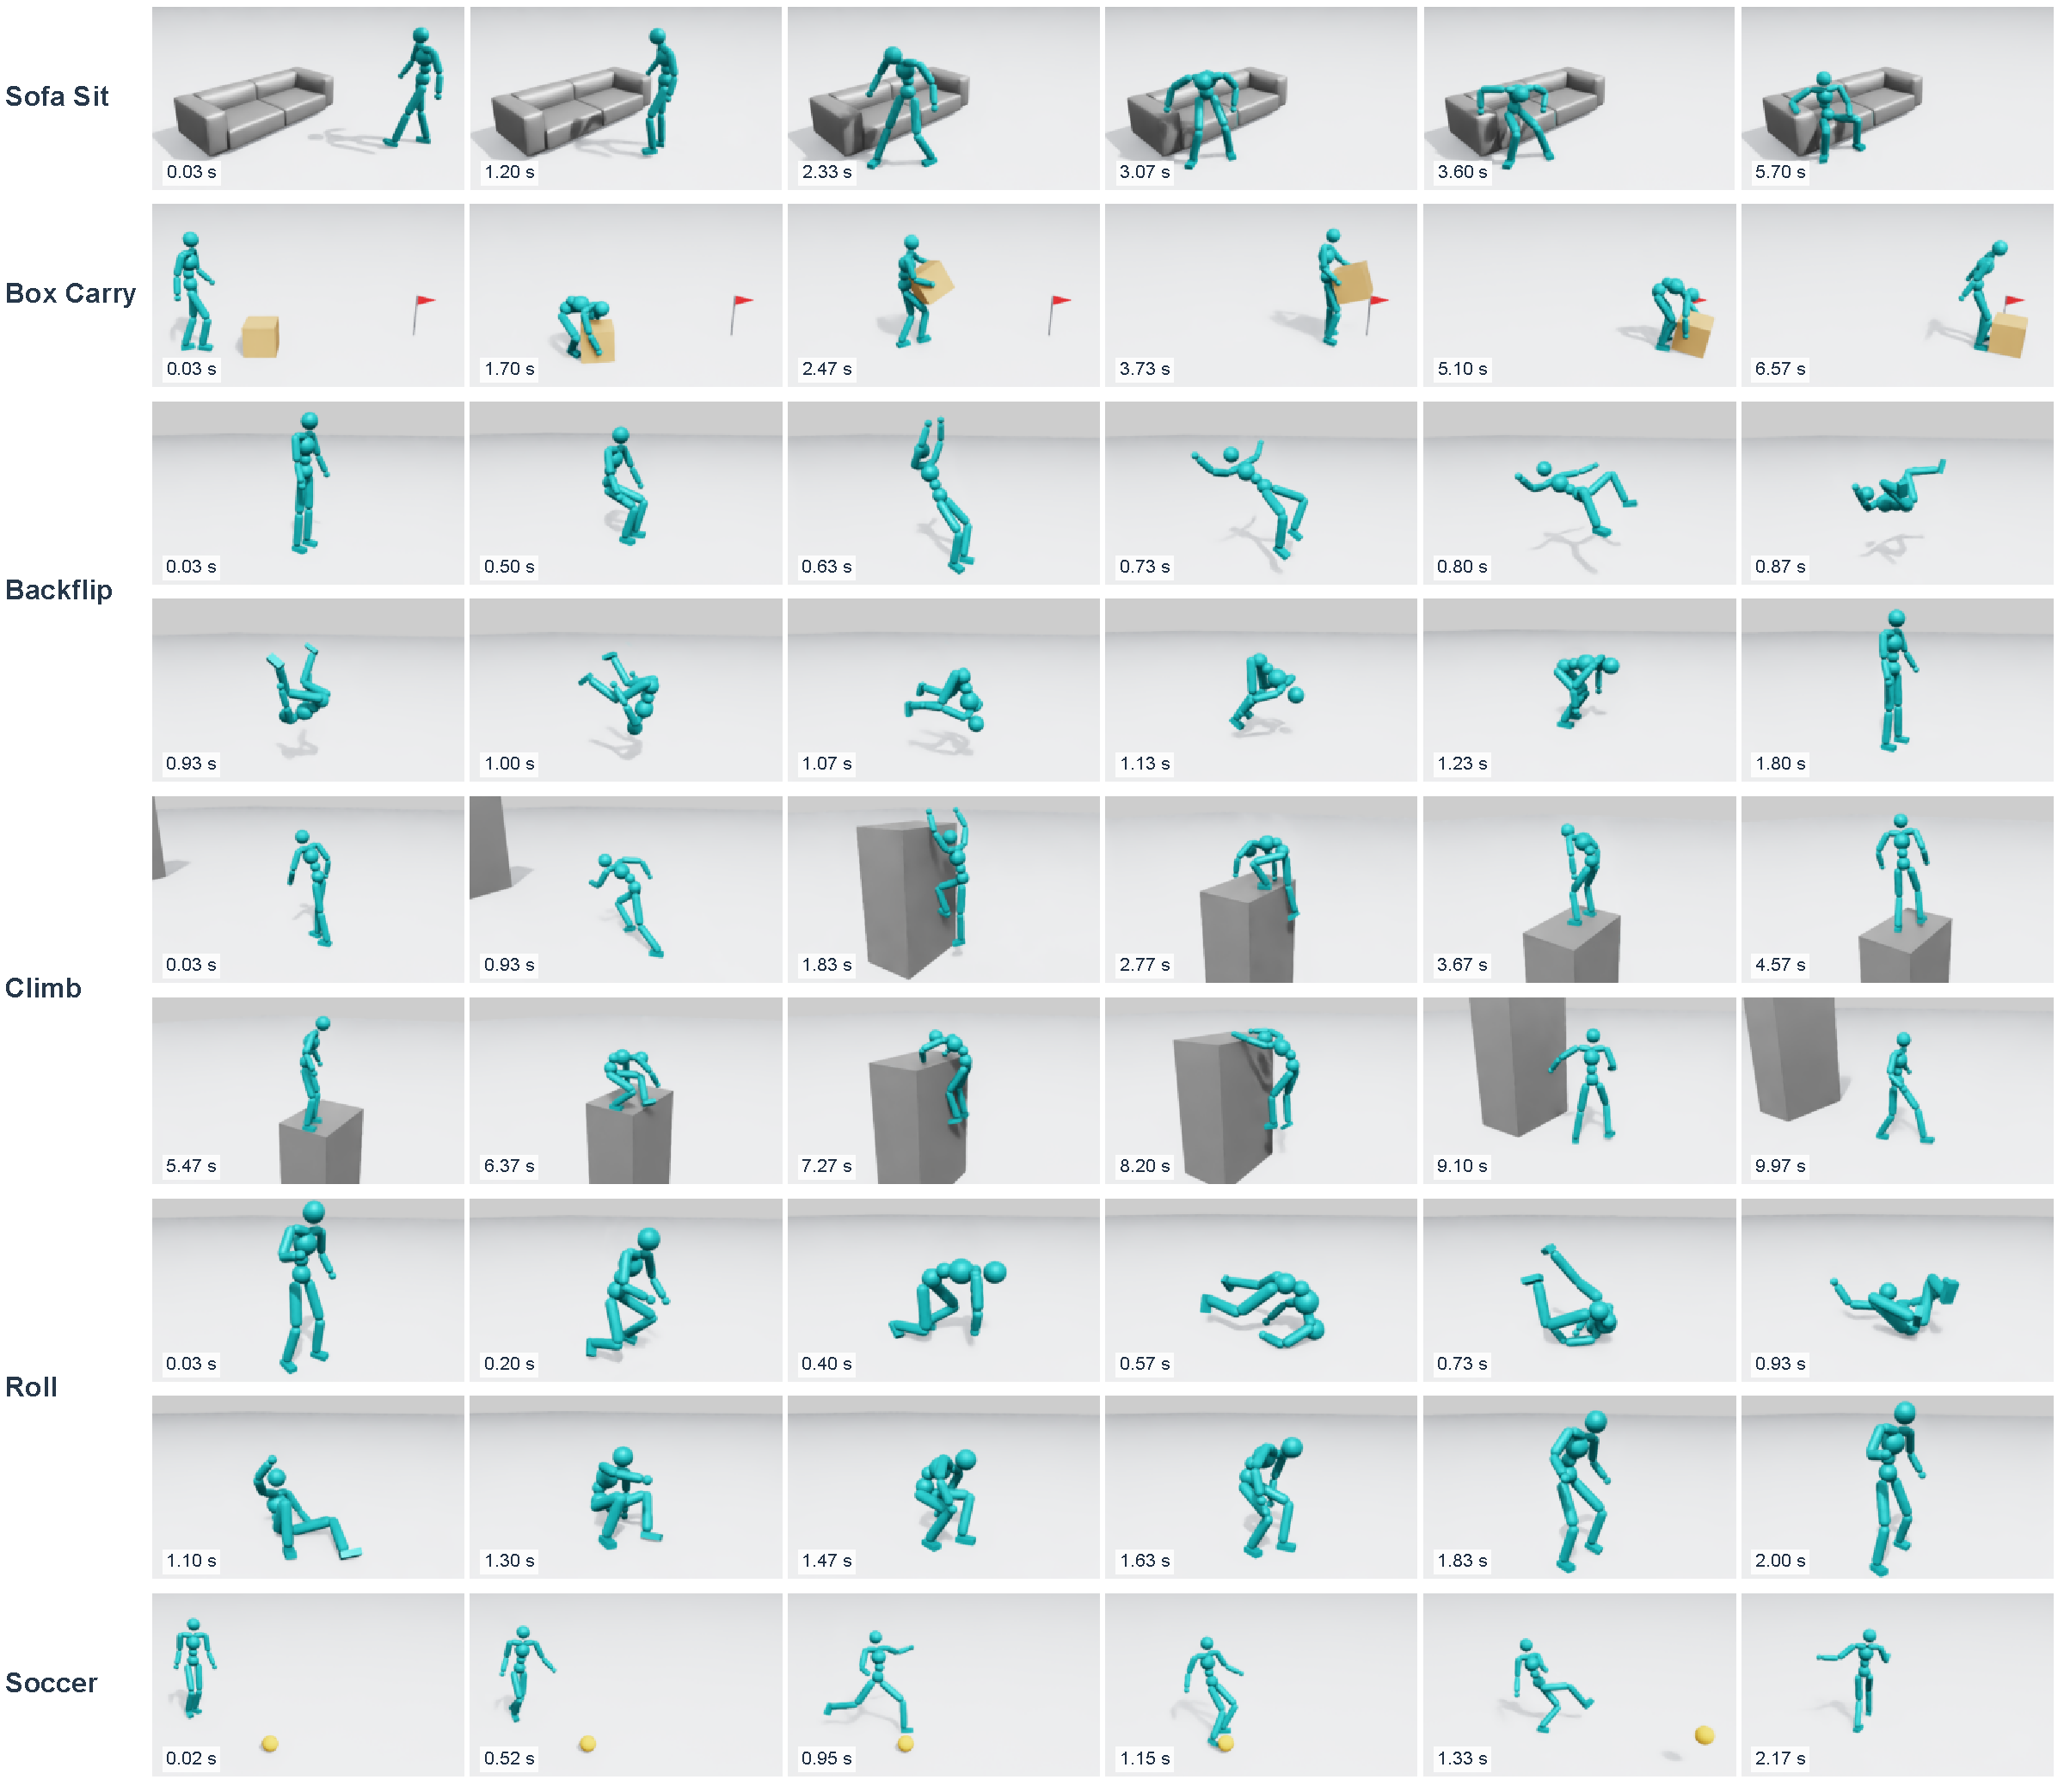
\includegraphics[width=0.97\textwidth]{figures/mira_rollout_screenshots.pdf}
\caption{Isaac Lab snapshots from policy rollouts. Sofa Sit, Box Carry, and
Soccer are additional interaction examples with six keyframes each.
Backflip, Climb, and Roll use twelve keyframes each. Backflip is sampled
more densely during the airborne phase.}
\label{fig:snapshots}
\end{figure*}

\begin{figure*}[!t]
\centering
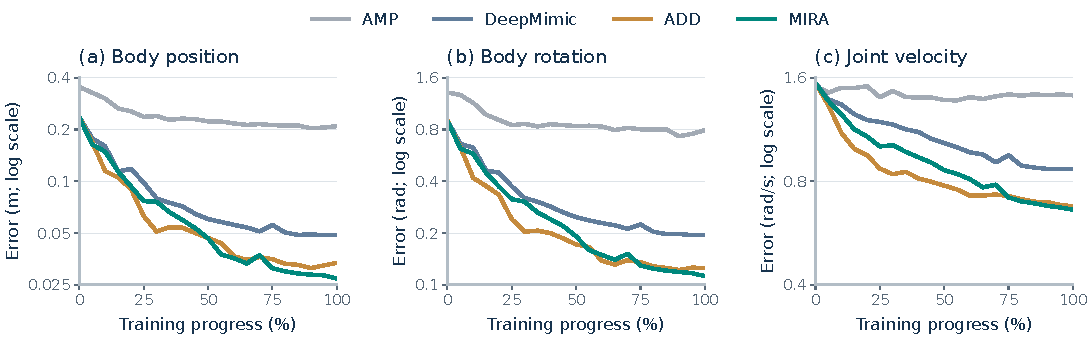
\includegraphics[width=0.97\textwidth]{figures/mira_tracking_curves.pdf}
\caption{Six-motion mean tracking curves from measured seed-0
reference-start tests. Progress is the fraction of each run's training
budget, as listed in Table~\ref{tab:main}.
Errors cover executed trajectory portions; lower is better.}
\label{fig:learning}
\end{figure*}

\begin{table*}[t]
\caption{Backflip component analysis at 2000 updates. Completion is
reported as a check or cross from the measured seed-0 reference-start test.
Errors of incomplete motions cover only the executed portion.
\textcolor{orange!70!black}{$\dagger$: Synthetic layout deviations;
additional seed repetitions remain pending.}
}
\label{tab:ablation}
\centering\scriptsize
\setlength{\tabcolsep}{3pt}
\resizebox{\textwidth}{!}{\begin{tabular}{lcccccccc}\toprule
Configuration & Root pos. & Root rot. & Body pos. & Body rot. & DoF vel. & Root vel. & Root ang. vel. & Complete \\
\midrule
\textbf{MIRA} & $0.0544\!\pm\!\textcolor{orange!70!black}{0.0033}^{\dagger}$ & $0.0303\!\pm\!\textcolor{orange!70!black}{0.0026}^{\dagger}$ & $0.0373\!\pm\!\textcolor{orange!70!black}{0.0023}^{\dagger}$ & $0.1701\!\pm\!\textcolor{orange!70!black}{0.0073}^{\dagger}$ & $0.9793\!\pm\!\textcolor{orange!70!black}{0.0425}^{\dagger}$ & $0.2760\!\pm\!\textcolor{orange!70!black}{0.0133}^{\dagger}$ & $0.2316\!\pm\!\textcolor{orange!70!black}{0.0098}^{\dagger}$ & $\checkmark$ \\
w/o Monotone Modeling & $0.1226\!\pm\!\textcolor{orange!70!black}{0.0057}^{\dagger}$ & $0.1270\!\pm\!\textcolor{orange!70!black}{0.0076}^{\dagger}$ & $0.0693\!\pm\!\textcolor{orange!70!black}{0.0034}^{\dagger}$ & $0.3061\!\pm\!\textcolor{orange!70!black}{0.0030}^{\dagger}$ & $1.7812\!\pm\!\textcolor{orange!70!black}{0.1119}^{\dagger}$ & $0.3729\!\pm\!\textcolor{orange!70!black}{0.0206}^{\dagger}$ & $0.9161\!\pm\!\textcolor{orange!70!black}{0.0338}^{\dagger}$ & $\checkmark$ \\
w/o Diagonal Norm. & $0.0609\!\pm\!\textcolor{orange!70!black}{0.0039}^{\dagger}$ & $0.1031\!\pm\!\textcolor{orange!70!black}{0.0020}^{\dagger}$ & $0.0596\!\pm\!\textcolor{orange!70!black}{0.0029}^{\dagger}$ & $0.2449\!\pm\!\textcolor{orange!70!black}{0.0132}^{\dagger}$ & $1.4464\!\pm\!\textcolor{orange!70!black}{0.0011}^{\dagger}$ & $0.2650\!\pm\!\textcolor{orange!70!black}{0.0102}^{\dagger}$ & $0.7879\!\pm\!\textcolor{orange!70!black}{0.0199}^{\dagger}$ & $\times$ \\
w/o Both Components & $0.0776\!\pm\!\textcolor{orange!70!black}{0.0021}^{\dagger}$ & $0.1158\!\pm\!\textcolor{orange!70!black}{0.0071}^{\dagger}$ & $0.0651\!\pm\!\textcolor{orange!70!black}{0.0020}^{\dagger}$ & $0.2767\!\pm\!\textcolor{orange!70!black}{0.0113}^{\dagger}$ & $1.4357\!\pm\!\textcolor{orange!70!black}{0.1134}^{\dagger}$ & $0.2815\!\pm\!\textcolor{orange!70!black}{0.0148}^{\dagger}$ & $0.6750\!\pm\!\textcolor{orange!70!black}{0.0283}^{\dagger}$ & $\times$ \\
\bottomrule\end{tabular}}
\end{table*}




\section{Experiments}

\subsection{Experimental Setup}
\label{sec:setup}
We evaluate MIRA on a $28$-DoF, $15$-body humanoid in Isaac Lab
\cite{mittal2023isaaclab,makoviychuk2021isaacgym}. The benchmark comprises
six skills: Roll, Climb, Backflip, Crawl, Get-Up, and Spin Kick. The main
base training budget is $2000$ policy updates with $8192$ parallel
environments and $32$ steps per update, corresponding to
$5.24\times10^8$ environment samples. The Climb extension is specified
in Table~\ref{tab:main}.
The simulator runs at $120\,\mathrm{Hz}$ and PD joint-position actions are
applied at $30\,\mathrm{Hz}$. MIRA uses the same configuration across motions
(Table~\ref{tab:config}), without a gradient penalty or an additional
handcrafted tracking reward.

Results use one training seed (seed~0) per configuration and deterministic
reference-start tests recorded during training. Additional training seeds
and a unified independent checkpoint evaluation remain \textbf{TODO}.

We report seven tracking errors: root position, root rotation, body position,
body rotation, joint velocity, root linear velocity, and root angular
velocity. Position errors use Euclidean distances; body positions are
expressed relative to the root. Rotation errors use quaternion geodesic
angles, with body orientations measured in world coordinates. Velocity
errors use mean absolute component differences. The environment's body
metrics average over its $15$ rigid bodies, while MIRA's input omits
duplicated root entries from the body groups. All errors are computed on
reference-aligned executed timesteps. Early-terminated trajectories are not
padded, so their errors must be interpreted together with completion.
The ablation table additionally marks whether each run reaches the full
motion horizon.

\subsection{Quantitative Comparison}
We compare MIRA with AMP, DeepMimic, and ADD. Table~\ref{tab:main} summarizes
the seven tracking errors, with all six motions weighted equally. The
table reports all four methods together and lists MIRA's per-motion
results. The learned skills are illustrated in Fig.~\ref{fig:snapshots}.
These measurements characterize the available seed-0 runs, rather than
establishing uniform superiority across motions or training seeds.

\subsection{Learning Dynamics}
\label{sec:learning}
Figure~\ref{fig:learning} reports body-position, body-rotation, and joint-velocity
errors during training. Every method is averaged equally over the same six
motions at equal fractions of each run's training budget. The four
algorithms use the same evaluation and aggregation protocol, exposing
differences in learning progress and final tracking accuracy. The curves
do not establish an improvement
on every motion or statistical significance across training seeds.

\subsection{Ablation Study}
\label{sec:ablation}
We examine two components on Backflip: \emph{Monotone Error Modeling} and
\emph{Diagonal Normalization}. Removing Monotone Error Modeling replaces
the physical error vector with the ADD-style $172$-dimensional signed
reference--policy differential, applies coordinate-wise normalization, and
allows signed network weights. The compatible diagonal normalization is
retained. Removing Diagonal Normalization preserves the physical error
input and nonnegative weights but removes the layer-wise normalization
during training. We also evaluate the configuration with both components
removed.

The binary classification objective, reward mapping, MixedELU activations,
hidden widths, PPO settings, and training budget are shared. Configurations
without diagonal normalization start from the corresponding normalized
model's effective initial weights. This avoids introducing an arbitrary
initial output-scale change. All variants retain the existing output-weight
regularizer. This penalty is constant for the unit-norm normalized scalar
head and becomes active when normalization is removed. Monotone Error
Modeling is evaluated as a joint representation
and constraint component, rather than an isolated dimensionality change.

Table~\ref{tab:ablation} reports tracking errors and whether the
reference-start evaluation reaches the full motion duration. Removing
Monotone Error Modeling preserves completion but increases all seven errors
in the available run. Both configurations without Diagonal Normalization
terminate early. These comparisons evaluate the components as implemented;
the additional seed repetitions remain pending.

To inspect discriminator behavior, Fig.~\ref{fig:diagnostics} shows sampled
input sensitivity, negative-sample logits, and numerically zero rewards.
Removing Diagonal Normalization is accompanied by increased sensitivity,
more negative scores, and reward saturation. These observations connect the
constraint to the reward's operating behavior, without attributing the
entire control gap to a single mechanism. The diagnostics use the measured
Backflip run and do not stand in for a six-motion result.

\FloatBarrier

% The final diagnostic shares the page with the conclusion and references.
\twocolumn[{
\begin{minipage}{\textwidth}
\MiraFigureType
\centering
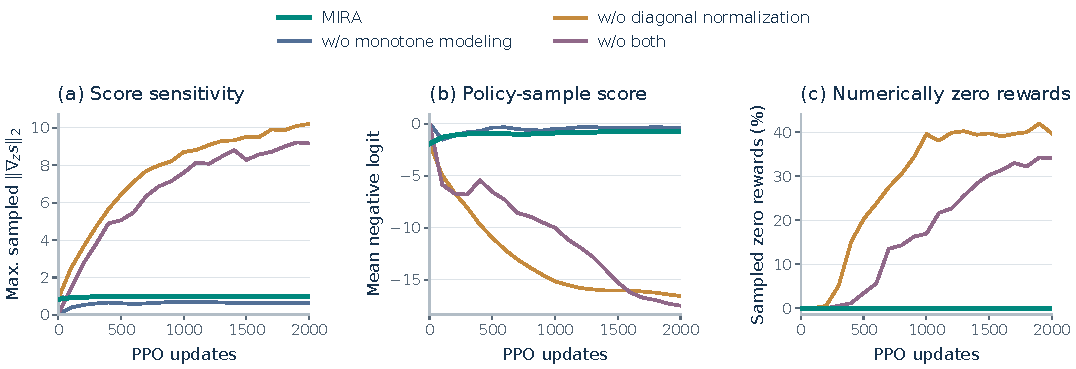
\includegraphics[width=0.97\textwidth]{figures/mira_discriminator_diagnostics.pdf}
\caption{Backflip discriminator diagnostics for the four ablations:
sampled maximum score-gradient norm (left), mean negative logit (middle),
and numerically zero rewards (right). Gradients use each model's normalized
coordinates and its own rollouts; they are local operating diagnostics,
not global bounds or common-state causal comparisons.}
\label{fig:diagnostics}
\vspace{12pt}
\end{minipage}
}]
